% analysis.tex

\chapter{Analysis}
\thispagestyle{chapterstart}

\section{Methodology}

In this analysis, we evaluate the side-channel resistance and performance of various masked implementations of the CRYSTALS-Dilithium digital signature scheme. Our methodology focuses on comparing key metrics across selected implementations to understand the trade-offs between security and efficiency, particularly in the context of embedded devices.

The main aspects considered are:

\begin{itemize}
    \item \textbf{Security Level}: The order of masking applied and the robustness against side-channel attacks.
    \item \textbf{Performance Metrics}: Execution time, cycle counts, and computational overhead introduced by the masking techniques.
    \item \textbf{Feasibility on Embedded Devices}: Practicality of implementations on resource-constrained platforms.
    \item \textbf{Implementation Techniques}: Specific masking schemes and optimizations employed to enhance security and performance.
    \item \textbf{Trade-offs}: Balancing security requirements with performance constraints.
\end{itemize}

We base our analysis on a selection of key papers that have contributed significantly to the field of side-channel resistant implementations of Dilithium.

\section{Selected Implementations}

\subsection{Efficient and Secure Masking of Dilithium}

Prest et al.\ introduce a first-order masked implementation of Dilithium, focusing on efficient techniques suitable for embedded devices. They address the challenges of masking lattice-based operations and aim to minimize the performance overhead associated with side-channel countermeasures.

\subsubsection{Security Level}

The implementation targets first-order side-channel resistance by applying masking to sensitive variables. The authors carefully identify the parts of the algorithm that require protection, such as the secret keys and intermediate computations involving these keys.

\subsubsection{Performance Metrics}

Key performance metrics reported include:

\begin{itemize}
    \item \textbf{Execution Time}: The masked implementation introduces an overhead of approximately $2\times$ compared to the unmasked version.
    \item \textbf{Cycle Counts}: Specific optimizations reduce the cycle counts for critical operations.
\end{itemize}

\subsubsection{Feasibility on Embedded Devices}

The authors demonstrate that their first-order masked implementation is practical on embedded platforms, achieving acceptable performance with minimal resource consumption.

\subsubsection{Implementation Techniques}

They employ specialized algorithms for masking polynomial arithmetic and optimize the implementation by minimizing the number of non-linear operations that require costly masking.

\subsection{Protecting Dilithium Against Leakage Revisited}

Azouaoui et al.\ revisit the masking of Dilithium by refining the sensitivity analysis and introducing efficient higher-order masking techniques. They provide implementations supporting masking orders up to $d = 8$.

\subsubsection{Security Level}

The implementations offer up to ninth-order side-channel resistance. The authors emphasize the importance of accurately identifying sensitive components to avoid unnecessary masking.

\subsubsection{Performance Metrics}

Performance improvements are achieved through:

\begin{itemize}
    \item \textbf{Optimized Gadgets}: New masking gadgets reduce the overhead of critical operations.
    \item \textbf{Randomized vs.\ Deterministic Signing}: Randomized signing shows significant performance gains over deterministic signing.
\end{itemize}

For first-order masking ($d=2$), the randomized implementation requires approximately 13.9 million cycles on an ARM Cortex-M4 microcontroller.

\subsubsection{Feasibility on Embedded Devices}

The implementations are practical on embedded devices for lower masking orders. The performance overhead increases with higher masking orders but remains manageable.

\subsubsection{Implementation Techniques}

Key strategies include:

\begin{itemize}
    \item \textbf{Refined Sensitivity Analysis}: Avoiding unnecessary masking to improve efficiency.
    \item \textbf{PINI-Compliant Gadgets}: Using Probe-Isolating Non-Interference (PINI) gadgets for secure and composable masking.
\end{itemize}

\subsection{Improved Gadgets for the High-Order Masking of Dilithium}

Coron et al.\ propose new masking gadgets to enhance the efficiency of high-order masking in Dilithium. They focus on reducing the complexity of critical operations and provide security proofs in the probing model.

\subsubsection{Security Level}

The gadgets are designed to be secure against high-order side-channel attacks, with proofs ensuring robustness in the $t$-probing model.

\subsubsection{Performance Metrics}

Significant performance improvements are reported for small masking orders:

\begin{itemize}
    \item \textbf{ShiftMod Gadget}: Reduces complexity of arithmetic shifts, improving efficiency.
    \item \textbf{Boolean-to-Arithmetic Conversion}: Achieves lower operation counts for small $n$.
\end{itemize}

However, the complexity increases exponentially with the masking order $n$, limiting practicality for higher orders.

\subsubsection{Feasibility on Embedded Devices}

For small masking orders, the implementations are feasible on embedded devices. The exponential complexity makes higher-order masking less practical on resource-constrained platforms.

\subsubsection{Implementation Techniques}

Innovations include:

\begin{itemize}
    \item \textbf{ShiftMod Gadget}: Efficient arithmetic shifts modulo $2q$.
    \item \textbf{Optimized Masking of Decompose Function}: Two methods providing efficiency gains.
\end{itemize}

\section{Comparative Analysis}

We compare the selected implementations based on the key metrics outlined in our methodology.

\subsection{Security Level and Side-Channel Resistance}

\begin{table}[h]
    \centering
    \caption{Security Levels of Implementations}
    \begin{tabular}{lcc}
        \toprule
        \textbf{Implementation} & \textbf{Masking Order} & \textbf{Targeted Security}                           \\
        \midrule
        Prest et al.\           & $d = 2$ (First-order)  & Protection against single-variable leakage           \\
        Azouaoui et al.\        & $d = 2$ to $d = 8$     & Higher-order side-channel resistance                 \\
        Coron et al.\           & Up to $d = 6$          & High-order security with proofs in $t$-probing model \\
        \bottomrule
    \end{tabular}
    \label{tab:security_levels}
\end{table}

\subsection{Performance Comparison}

\begin{table}[h]
    \centering
    \caption{Performance Metrics of Implementations (First-Order Masking)}
    \begin{tabular}{lcc}
        \toprule
        \textbf{Implementation} & \textbf{Execution Time}     & \textbf{Cycle Counts}                 \\
        \midrule
        Prest et al.\           & $\approx 2\times$ overhead  & Reduced cycles for critical ops       \\
        Azouaoui et al.\        & 13.9 million cycles (rand.) & Optimized gadgets improve performance \\
        Coron et al.\           & Improved for small $n$      & Low operation counts for key gadgets  \\
        \bottomrule
    \end{tabular}
    \label{tab:performance_metrics}
\end{table}

\subsection{Scalability with Masking Order}

\begin{itemize}
    \item \textbf{Prest et al.}: Focuses on first-order masking; higher orders not addressed.
    \item \textbf{Azouaoui et al.}: Provides scalable implementations up to $d = 8$; performance overhead increases with $d$.
    \item \textbf{Coron et al.}: Efficient for small $n$; exponential complexity limits higher-order practicality.
\end{itemize}

\subsection{Feasibility on Embedded Devices}

All implementations consider embedded platforms:

\begin{itemize}
    \item \textbf{Prest et al.}: Demonstrates practicality for first-order masking.
    \item \textbf{Azouaoui et al.}: Shows acceptable performance for higher-order masking on devices like ARM Cortex-M4.
    \item \textbf{Coron et al.}: Suitable for small masking orders; higher orders may not be feasible due to resource constraints.
\end{itemize}

\subsection{Implementation Techniques and Optimizations}

\begin{table}[h]
    \centering
    \caption{Implementation Techniques}
    \begin{tabular}{l p{10cm}}
        \toprule
        \textbf{Implementation} & \textbf{Techniques and Optimizations}                                                                           \\
        \midrule
        Prest et al.\           & Specialized algorithms for masking polynomial arithmetic; focus on minimizing non-linear operations.            \\
        Azouaoui et al.\        & Refined sensitivity analysis; PINI-compliant gadgets; performance gains from randomized signing.                \\
        Coron et al.\           & Introduction of ShiftMod gadget; optimized Boolean-to-arithmetic conversions; security proofs in probing model. \\
        \bottomrule
    \end{tabular}
    \label{tab:implementation_techniques}
\end{table}

\subsection{Trade-offs Between Security and Performance}

\begin{itemize}
    \item \textbf{Prest et al.}:
          \begin{itemize}
              \item Prioritizes performance for first-order masking.
              \item Accepts that higher-order masking would incur significant overhead.
          \end{itemize}
    \item \textbf{Azouaoui et al.}:
          \begin{itemize}
              \item Balances higher-order security with optimized performance.
              \item Randomized signing improves both security and efficiency.
          \end{itemize}
    \item \textbf{Coron et al.}:
          \begin{itemize}
              \item Provides strong security proofs and efficiency for small $n$.
              \item Acknowledges limitations for higher masking orders due to complexity.
          \end{itemize}
\end{itemize}

\subsection{Visual Comparison of Performance}

We present a comparative visualization of the operation counts for the Boolean-to-Arithmetic conversion, a critical operation in masked implementations.

\begin{figure}[h]
    \centering
    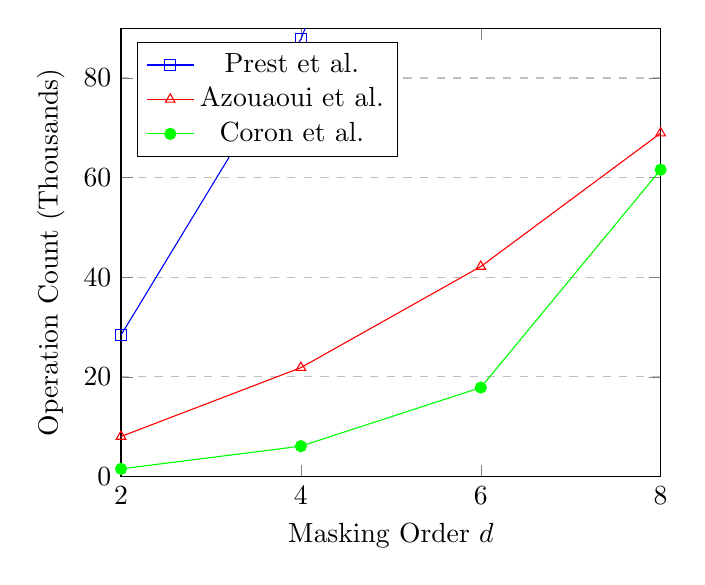
\begin{tikzpicture}
        \begin{axis}[
                xlabel={Masking Order $d$},
                ylabel={Operation Count (Thousands)},
                xmin=2, xmax=8,
                ymin=0, ymax=90,
                xtick={2,4,6,8},
                ytick={0,20,40,60,80},
                legend pos=north west,
                ymajorgrids=true,
                grid style=dashed,
            ]

            \addplot[
                color=blue,
                mark=square,
            ]
            coordinates {
                    (2, 28.41)
                    (4, 87.82)
                    (6, 178.25)
                    (8, 302.35)
                };
            \addlegendentry{Prest et al.}

            \addplot[
                color=red,
                mark=triangle,
            ]
            coordinates {
                    (2, 8.04)
                    (4, 21.86)
                    (6, 42.16)
                    (8, 68.94)
                };
            \addlegendentry{Azouaoui et al.}

            \addplot[
                color=green,
                mark=*,
            ]
            coordinates {
                    (2, 1.54)
                    (4, 6.10)
                    (6, 17.86)
                    (8, 61.60)
                };
            \addlegendentry{Coron et al.}

        \end{axis}
    \end{tikzpicture}
    \caption{Operation Counts for Boolean-to-Arithmetic Conversion at Different Masking Orders}
    \label{fig:b2a_comparison}
\end{figure}

The figure illustrates that Coron et al.'s method has lower operation counts for small $d$, but the counts increase rapidly for higher $d$.

\section{Summary and Conclusions}

Our analysis highlights the following:

\begin{itemize}
    \item \textbf{Prest et al.} offer efficient first-order masking suitable for applications where minimal overhead is acceptable.
    \item \textbf{Azouaoui et al.} provide scalable higher-order masking with performance optimizations, particularly through randomized signing.
    \item \textbf{Coron et al.} introduce innovative gadgets that improve efficiency for small masking orders but face limitations for higher orders.
\end{itemize}

The choice of implementation depends on application requirements:

\begin{itemize}
    \item For applications requiring only first-order protection, Prest et al.'s methods are appropriate.
    \item For stronger security needs with acceptable performance overhead, Azouaoui et al.'s implementations are suitable.
    \item For strong security proofs and efficiency at low masking orders, Coron et al.'s methods offer advantages.
\end{itemize}

\section{Recommendations for Practical Deployment}

When deploying side-channel resistant implementations of Dilithium, consider:

\begin{itemize}
    \item \textbf{Security Requirements}: Assess the required masking order based on the threat model.
    \item \textbf{Performance Constraints}: Evaluate the available computational resources to determine feasible masking techniques.
    \item \textbf{Randomized vs.\ Deterministic Signing}: Use randomized signing when acceptable to leverage performance benefits.
    \item \textbf{Implementation Complexity}: Balance the complexity of advanced masking gadgets with the benefits they provide.
\end{itemize}

Future work may focus on developing methods that reduce the complexity of high-order masking, making them more practical for a wider range of applications.

